\section{Triangle-Feed Antenna}

In Chapter~\ref{cha:prototypes} it was found that the triangle-feed antenna design was found to have the highest efficiency and to be the most sweepable of the designs. For this reason, the triangle-feed design has been chosen as the first design to move to the printed circuit board with the WiSpry tuners installed. 

\begin{figure}[htbp]
    \centering
    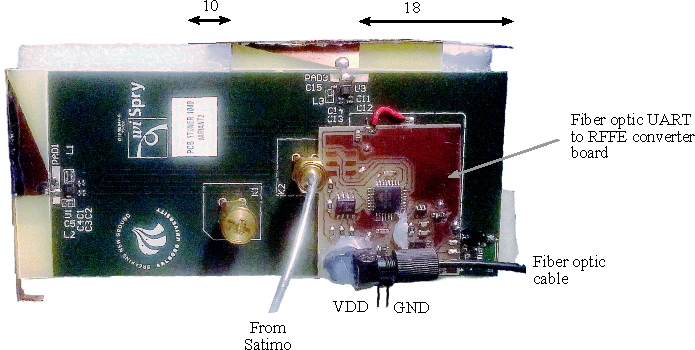
\includegraphics{img/tech_sol/pcb_trianglefeed/pcb_enh}\\[2em]
    \footnotesize
    \begin{tabular}{|l|l|l|l|}
        \hline
        & $C_{\text{series}}$ & $L_{\text{shunt}}$ & $C_{\text{shunt}}$ \\
        \hline
        Top antenna & \SI{8.2}{pF} & \SI{3.3}{nH} & 0.6--\SI{6}{pF} \\
        Side antenna & \SI{4.7}{pF} & \SI{1.0}{nH} & 1.2--\SI{12}{pF} \\
        \hline
    \end{tabular}
    \caption{Triangle-feed antenna on a PCB with two WiSpry tuners. The location of the side-feed is different from the prototype and for this reason, the side antenna has slightly different dimensions. The changes from Figure~\ref{fig:ant2technical} is noted on the figure.}
    \label{fig:triang_pcb_enh}
\end{figure}

The antennas are shown in Figure~\ref{fig:triang_pcb_enh}. The side antenna has been moved further towards the top to align with the feed. Extra length has been added by the end of the triangle, as this results in a greater bandwidth around \SI{1800}{MHz}.

The antenna is tuned using the fiber-optic RFFE adapter described in Appendix~\ref{cha:optical_rffe_comm}.

\begin{figure}[htbp]
    \centering
    \begin{subfigure}{0.49\linewidth}
        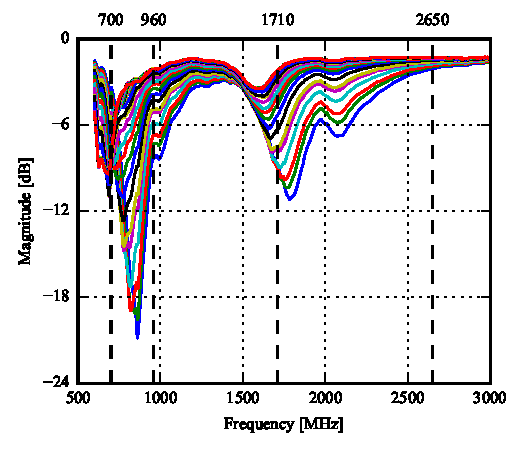
\includegraphics{img/tech_sol/pcb_trianglefeed/S11}
        \caption{S11.}
    \end{subfigure}
    \hfill
    \begin{subfigure}{0.49\linewidth}
        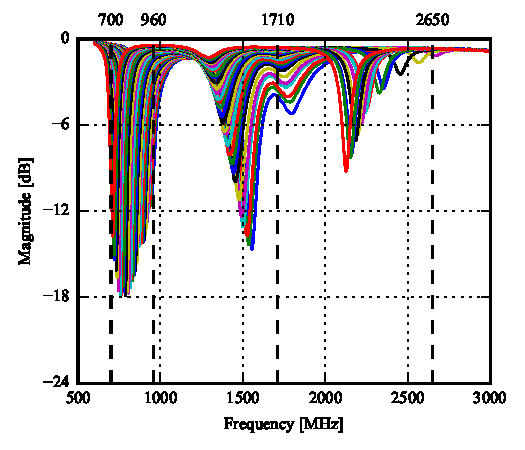
\includegraphics{img/tech_sol/pcb_trianglefeed/S22}
        \caption{S22.}
    \end{subfigure}
    \\
    \begin{subfigure}{0.49\linewidth}
         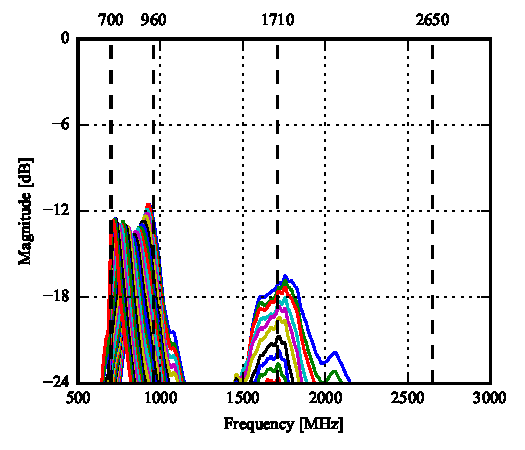
\includegraphics{img/tech_sol/pcb_trianglefeed/S21}
         \caption{S21.}
    \end{subfigure}
    \caption{S-parameters of the triangle-feed antenna with tuners. The first sixteen values, the two tuners are tracking. After this, only the side tuner is altered.}
    \label{fig:triang_pcb_sparams}
\end{figure}

The S-parameters sweeps are shown in Figure~\ref{fig:triang_pcb_sparams}. As it is seen, the high end of the high band -- near \SI{2.6}{GHz} -- does not resonate as well as the prototype. However, the low band can be covered quite well for both the top and the side antenna.

\begin{figure}[htbp]
    \centering
    \begin{subfigure}{0.49\linewidth}
        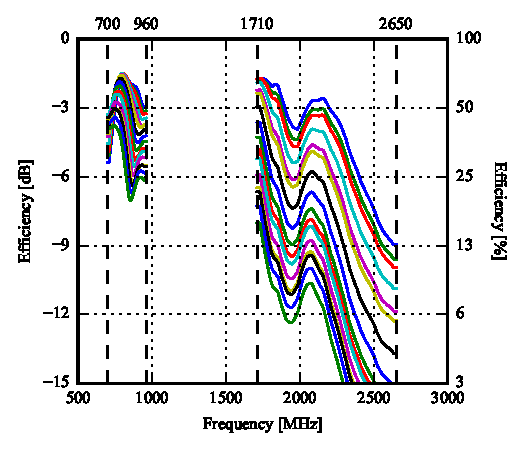
\includegraphics{img/tech_sol/pcb_trianglefeed/efficiency_top}
        \caption{Top antenna.}
    \end{subfigure}
    \hfill
    \begin{subfigure}{0.49\linewidth}
        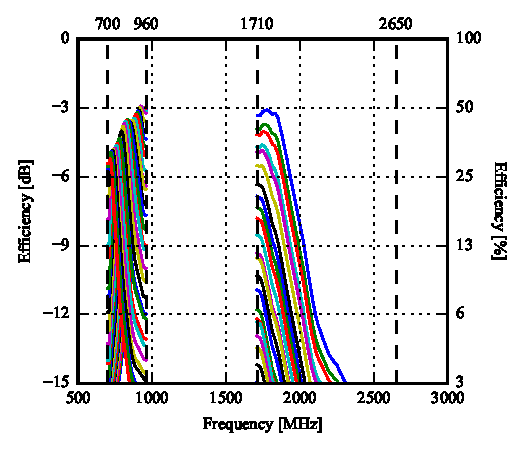
\includegraphics{img/tech_sol/pcb_trianglefeed/efficiency_side}
        \caption{Side antenna.}
    \end{subfigure}
    \caption{Total efficiency of the triangle-feed antennas with tuners.}
    \label{fig:triang_pcb_eff}
\end{figure}

The total efficiency is plotted in Figure~\ref{fig:triang_pcb_eff}. The efficiency, likewise, reflects that resonance is lacking near \SI{2.6}{GHz}, so the mismatch loss is quite severe -- especially for the side antenna. The low band looks acceptable for both antennas as the top antenna has a total efficiency above \SI{-3.1}{dB} and the side antenna has a total efficiency above \SI{-5.5}{dB}.
